\documentclass{beamer}
%\usetheme{Ilmenau}
%\usecolortheme{beaver}

\usepackage[slovak,american]{babel}
\usepackage[utf8]{inputenc}
\usepackage{graphicx}
\usepackage{adjustbox}
 \usepackage{xcolor}
 
 \newsavebox\MBox
\newcommand\Cline[2][red]{{\sbox\MBox{$#2$}%
  \rlap{\usebox\MBox}\color{#1}\rule[-2.2\dp\MBox]{\wd\MBox}{1pt}}}

%\usefonttheme{serif}

%\definecolor{UKOrange}{HTML}{ef9424} %
\definecolor{UKOrange}{HTML}{7a2c18} %
\definecolor{UKBrown}{HTML}{a96d5e} %
\definecolor{UKLight}{HTML}{d8b6ab} %
\definecolor{UKDark}{HTML}{7a4f44}
\definecolor{UKDarker}{HTML}{4d312b} 
\definecolor{UKDarkest}{HTML}{2e1e1a}
\definecolor{UKRed}{HTML}{bf1f1c}

\setbeamertemplate{footline}[frame number]{}
\setbeamertemplate{navigation symbols}{}

%\usecolortheme{beaver}
\setbeamertemplate{itemize item}[square]
\setbeamercolor{itemize item}{fg = UKBrown}
\setbeamercolor{itemize subitem}{fg = UKLight}
\setbeamercolor{enumerate item}{fg = UKDark}

\setbeamercolor{footnote}{fg=UKLight}
\setbeamercolor{footnote mark}{fg=UKLight}
\setbeamerfont{footnote}{size=\tiny}
\renewcommand\footnoterule{}

\usetheme{default}
\beamertemplatenavigationsymbolsempty
\setbeamercolor{title}{fg=white, bg=UKBrown}
\setbeamercolor{frametitle}{fg=white, bg=UKBrown}
\setbeamercolor{block title}{bg=UKBrown, fg= white}
\setbeamercolor{block body}{bg =UKLight, fg = UKDarkest}

\setbeamercolor{block title alerted}{bg=UKOrange, fg= white}
\setbeamercolor{block body alerted}{bg =UKLight, fg = UKDarkest}


%\setbeamercolor{section in toc}{fg = UKBrown}
%\setbeamercolor{section in toc}{fg = UKDarkest}

% odstrani gulicky
\renewcommand*{\slideentry}[6]{}

\useoutertheme[subsection=false]{miniframes}
\AtBeginSection[]{\subsection{}}

\setbeamercolor{below lower separation line head}{bg=UKDark}
\addtobeamertemplate{headline}{}{%
  \begin{beamercolorbox}[colsep=0.5pt]{below lower separation line head}
  \end{beamercolorbox}
}
%\setbeamercolor*{mini frame}{fg=white,bg=UKRosy}
\setbeamercolor{section in head/foot}{fg=UKLight, bg=UKDark}

\usepackage{etoolbox}
\makeatletter
\preto{\@verbatim}{\topsep=0pt \partopsep=0pt }
\makeatother

%\setbeamertemplate{itemize/enumerate body begin}{\normalsize}
%\setbeamertemplate{itemize/enumerate subbody begin}{\normalsize}




%\newcommand{\codeblock}[2]{ \begin{block}{#1} \begin{verbatim}#2\end{verbatim}\end{block}}

%\defbeamertemplate*{title page}{customized}[1][]
%{
%  \begin{centering}
%    \begin{beamercolorbox}[sep=8pt,center]{title}
%      \usebeamerfont{title}\inserttitle
%    \end{beamercolorbox}
%  \end{centering}
%  \bigskip
%
%\begin{columns}[onlytextwidth,T]
%
%
%  \column{27mm}
%  \includegraphics[width=27mm]{images/logoFMFI.png}
%  
%  \column{\dimexpr\linewidth-54mm-6mm}
%  \centering
%  \vspace{5mm}  
%  \usebeamerfont{author}\insertauthor\par
%  \vspace{5mm}
%  \usebeamerfont{institute}\insertinstitute\par
%
%  \column{27mm}
%  \includegraphics[width=27mm]{images/logoUK.png}  
%\end{columns}
%\centering
%\vspace{7mm}
%  \usebeamerfont{date}\insertdate\par
%}

\DeclareMathOperator*{\argmin}{arg\,min}
\newcommand{\e}[1]{$\cdot 10^{#1}$}

%\newcommand{\codeblock}[2]{ \begin{block}{#1} \begin{verbatim}#2\end{verbatim}\end{block}}



\title[4. cvičenie]{Advanced Image Processing - Camera calibration and histograms}
\author[Kocur]{Ing. Viktor Kocur \\{\small viktor.kocur@fmph.uniba.sk}}
\institute{DAI FMFI UK}
\date{16.10.2019}

\begin{document}
\selectlanguage{slovak}

\begin{frame}
  \titlepage
\end{frame}

\section{Calibration}
\subsection{Intrinsic parameters}
\begin{frame}
\frametitle{Calibration process}
\begin{block}{Calibration pattern}
For Matlab calibration a checkerboard calibration pattern is used. It is possible to use a different pattern, but its detection has to be implemented. The whole calibration pattern has to be visible in the photos.
\end{block}

\begin{alertblock}{Taking photos}
When taking photos it is important to not change the camera configuration. It is therefore necessary to turn off features such as autofocus and to not use zoom. Such changes can change some of the intrinsic parameters of the camera.
\end{alertblock}
\end{frame}

\begin{frame}
\frametitle{Calibration App}
\begin{block}{cameraParams}
We will use the Matlab Calibration Map to obtain the camera parameters via the struct cameraParams.
\end{block}

\begin{center}
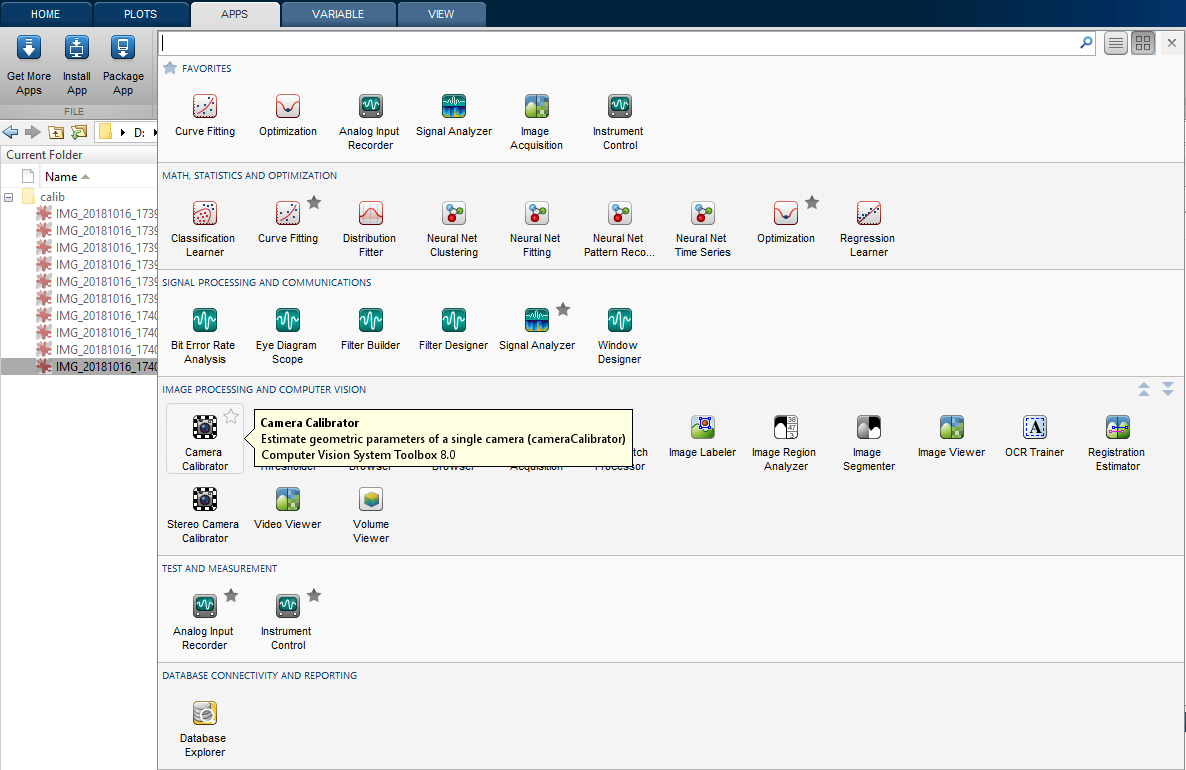
\includegraphics[width=0.7\textwidth]{calib_app.png}
\end{center}
\end{frame}

\subsection{Extrinsic parameters}
\begin{frame}
\frametitle{Image processing}
\begin{block}{undistort}
[im, newOrigin] = undistortImage(I, cameraParams) - returns image without distortion. newOrigin indicates the shift of origin between the coordinate system in the image and the undistorted image. In case of this value being [0, 0] it can be ignored.
\end{block}

\begin{block}{Exercise}
Display the undistorted image for one of the captured images. Try to use undistortImage(I, cameraParams, 'OutputView', 'full').
\end{block}

\end{frame}

\begin{frame}
\frametitle{Pattern detection}
\begin{block}{detectCheckerboardPoints}
[imagePoints, boardSize] = detectCheckerboardPoints(im) - returns positions of the corners in the calibration pattern
\end{block}

\begin{alertblock}{detectCheckerboardPoints}
If there was a shift of the origin in the undistortion step it is necessary to shift all of these points with the new origin, e.g. imagePoints = imagePoints + newOrigin
\end{alertblock}

\begin{block}{generateCheckerboardPoints}
worldPoints = generateCheckerboardPoints(boardSize, squareSize) - returns the positions of the points in real world coordinates. The parameter squareSize indicates the size of the square in millimeters.
\end{block}
\end{frame}

\begin{frame}
\frametitle{Extrinsic parameters}

\begin{block}{extrinsics}
[R, t] = extrinsics(imagePoints, worldPoints, cameraParams) - returns the rotation matrix R and the translation vector t for the given pairs of points and intrinsic camera parameters.
\end{block}

\begin{block}{Note}
If we try to apply this to an image we used in the app it is possible to obtain these values from the cameraParams struct.
\end{block}
\end{frame}

\begin{frame}
\frametitle{Point transformation}
\begin{block}{pointsToWorld}
pointsToWorld(cameraParams, R, t, imPoints) - returns the coordinates of the imPoints in the coordinate system of the plane of the calibration pattern. The arguments are the camera parameter struct, the rotation matrix, the translation vector and the points in the coordinate system of the image. 
\end{block}

\begin{alertblock}{Pozor!}
If we use imPoints from the ginput() function it is important to correct for the origin shift by adding the newOrigin value,
\end{alertblock}

\begin{block}{Exercise}
Use ginput and measure dimensions of an object in the image and check if this measurement corresponds to real world dimensions of the object.
\end{block}
\end{frame}

\section{Intensity}
\subsection{Histogram}
\begin{frame}
\frametitle{Histogram}
\begin{block}{imhist}
imhist(I) - displays the histogram, in case the output is directed to a variable the histogram is not shown and the values are stored in the variable as a vector.
\end{block}

\begin{block}{Exercise}
Convert the zatisie.jpg to grayscale (rgb2gray function). In its histogram we can see three peaks. Change the image so that the values belonging to just one of the three peaks are fully white (maximum intensity).
\end{block}
\end{frame}

\subsection{Intensity processing}
\begin{frame}
\frametitle{Intensity processing}
\begin{block}{Gamma correction}
Contrast in the image can be changed with the gamma correction: $i_{out} = A \cdot i^{\gamma}$, where $i$ are the intensities of the pixels of the image. The intensity values are expected to be between 0 and 1!
\end{block}

\begin{block}{Linear expansion}
To linearnly expand the intensity we can use the following:
\begin{equation*}
i_{out} = \frac{i - min(I)}{max(I) - min(I)},\end{equation*}
where $i$ are intensity values of the pixels and $I$ is the set of all the intensities in the image. We expect the values to be between 0 and 1.
\end{block}
\end{frame}

\begin{frame}
\frametitle{Histogram equalization}
\begin{block}{Equalization}
Histogram equalization is a method to change the intensity values in the image in a way that results in the most balanced histogram (closest to the uniform distribution).
\end{block}

\begin{block}{histeq}
histeq(I) - returns the image after histogram equalization.
\end{block}

\begin{block}{Exercise}
For the image krajinka.jpg use all of the 3 methods to change the intensity values. Display both the image and the corresponding histograms.
\end{block}
\end{frame}

\subsection{Thresholding}
\begin{frame}
\frametitle{Thresholding}
\begin{block}{imbinarize}
imbinarize(I) - returns the binarized image using the Otsu method.
\end{block}

\begin{block}{imbinarize}
imbinarize(I, t) - returns the binarized image with the threshold t.
\end{block}

\begin{block}{Exercise}
Try to use thresholding on images coins.png, qr.jpg a zatisie.jpg.
\end{block}
\end{frame}

\begin{frame}
\frametitle{Adaptive thresholding}
\begin{block}{imbinarize}
imbinarize(I, 'adaptive') - returns binarized image using adaptive thresholding.
\end{block}

\begin{block}{Exercise}
Try adaptive thresholding for the images coins.png a qr.jpg.
\end{block}
\end{frame}


\end{document}